\section{Auswertung}

\subsection{Messung der geometrischen Abmessungen}
Zunächst wurden die Abmessungen (Dicke $d$, Länge $l$, Breite $b$) der Proben aufgenommen. Die Werte
werden im Folgenden als fehlerfrei angenommen. Für die Kupferprobe wurden folgende Werte gemessen:
\begin{align}
  \begin{aligned}
    d_{Cu} &= 18 \si{\micro \meter} \\ %\SI verwenden
    l_{Cu} &= 28.05 \si{\milli \meter}\\ %\SI verwenden
    b_{Cu} &= 25.03 \si{\milli \meter} %\SI verwenden
        \label{eq: abmessungen_kupfer}
      \end{aligned}
\end{align}
Hierbei wurde der Wert für $d_{Cu}$ der Aufschrift auf der Apparatur entnommen.
Entsprechend für die Zinkprobe:

\begin{align}
  \begin{aligned}
    d_{Zn} &= 0.15 \si{\milli \meter} \\ %\SI verwenden
    l_{Zn} &= 43.00 \si{\milli \meter}\\
    b_{Zn} &= 25.50 \si{\milli \meter}
        \label{eq: abmessungen_zink}
      \end{aligned}
\end{align}



\subsection{Widerstandsmessung}
Für die Proben Zink und Kupfer wurde jeweils die Spannung in Abhängigkeit vom Strom gemessen. Die Messwerte befinden sich
in den Tabellen \ref{tab: uri_zink} und \ref{tab: uri_kupfer}.

\begin{minipage}{\textwidth}
 \begin{tabular}{S S } 
 \toprule  
 {$I$ in $\si{\ampere}$} & {$U$ in $\si{\volt}$}   \\ 
\midrule  
 0.0 & 0.0  \\ 
0.8 & 6.6  \\ 
1.6 & 12.5  \\ 
2.4 & 18.6  \\ 
3.2 & 24.7  \\ 
4.0 & 30.8  \\ 
4.8 & 37.0  \\ 
5.6 & 43.3  \\ 
6.4 & 49.6  \\ 
7.2 & 55.6  \\ 
8.0 & 63.4  \\ 
\bottomrule 
 \end{tabular} 
 \caption{Zinkprobe: Messung der Spannung in Abhängigkeit vom Strom } 
 \label{tab: uri_zink}
\hfill
\begin{table} 
\centering 
\caption{Kupferprobe: Messung der Spannung in Abhängigkeit vom Strom } 
\label{tab: uri_kupfer} 
\begin{tabular}{S S } 
\toprule  
{$I$ in $\si{\ampere}$} & {$U$ in $\si{\volt}$}   \\ 
\midrule  
 0.0  & 0.0\\ 
1.0  & 7.8\\ 
2.0  & 15.5\\ 
3.0  & 23.2\\ 
4.0  & 31.0\\ 
5.0  & 38.5\\ 
6.0  & 46.3\\ 
7.0  & 53.8\\ 
8.0  & 61.5\\ 
9.0  & 68.8\\ 
10.0  & 76.5\\ 
\bottomrule 
\end{tabular} 
\end{table}
\end{minipage}

Die Auftragung der Messwerte sowie die Regressionsgeraden sind in den Abbildungen \ref{fig: uri_zink} und \ref{fig: uri_kupfer} illustriert.
Als Regressionsparamter für die Steigungen, die den Widerständen entsprechen, ergeben sich die Werte:
\begin{equation}
  R_{Cu} = (7.64 \pm 0.02)\si{\milli \ohm} \quad \quad R_{Zn} = (7.80 \pm 0.06)\si{\milli \ohm}%\SI verwenden
  \label{eq: widerstand}
\end{equation}
\FloatBarrier
\begin{figure}
  \centering
  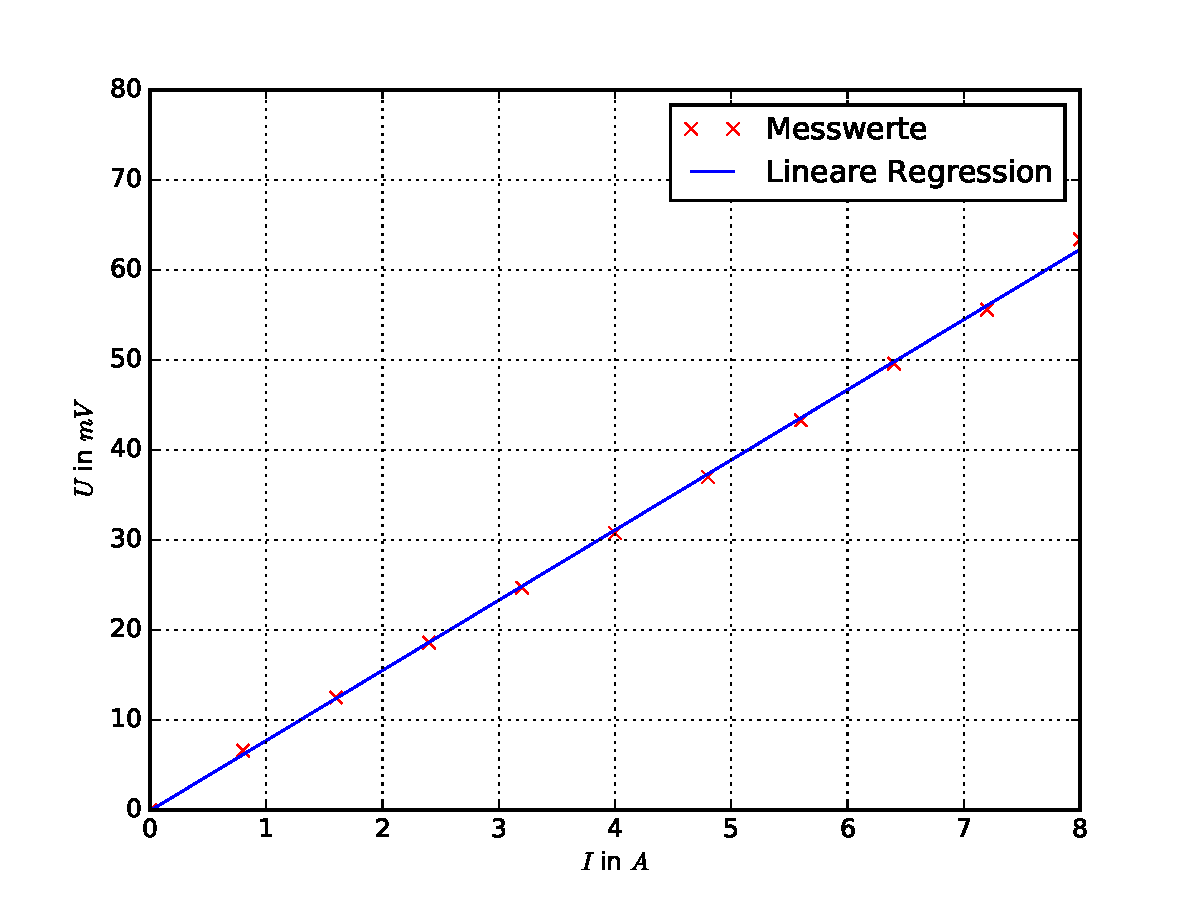
\includegraphics[width=0.7\textwidth]{pics/uri_zink.pdf}
  \caption{Zinkprobe Verlauf der Spannung in Abhängigkeit vom Strom}
  \label{fig: uri_zink}
\end{figure}
\begin{figure}
  \centering
  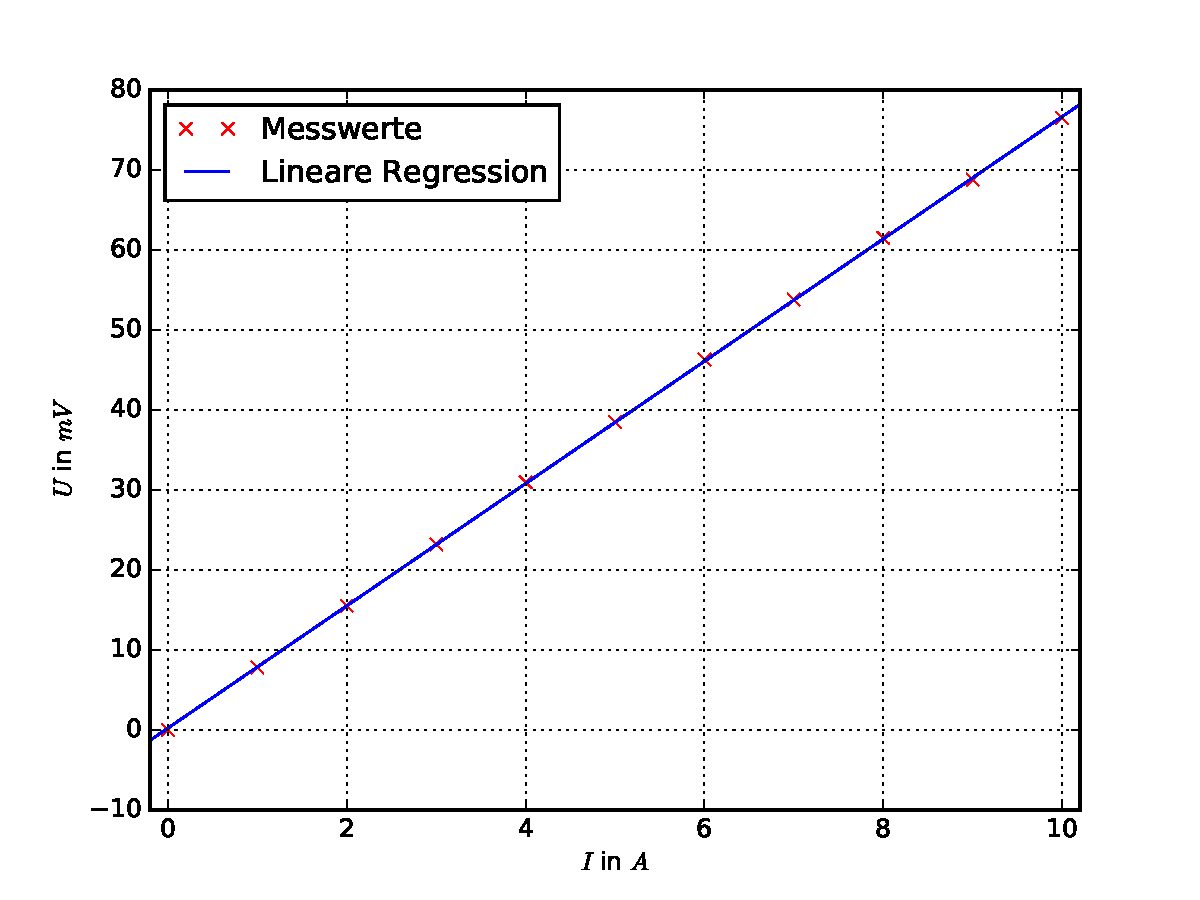
\includegraphics[width=0.7\textwidth]{pics/uri_kupfer.pdf}
  \caption{Kupferprobe Verlauf der Spannung in Abhängigkeit vom Strom}
  \label{fig: uri_kupfer}
\end{figure}



\subsection{Magnetfeldmessung}
Die Werte aus der Messung des Magnetfeldes in Abhängigkeit vom Spulenstrom sind in Tabelle \ref{tab: hysterese} einzusehen.
Hierbei entsprechen $B_{wachsend}$ bzw. $B_{fallend}$ den gemessenen magnetischen Flussdichten bei wachsendem
bzw. fallendem Spulenstrom.
Die graphische Darstellung (Abbildung \ref{fig: hysterese}) zeigt, dass die Hysterese-Effekte vernachlässigbar sind. Für
spätere Berechnungen soll der Zusammenhang zwischen dem ansteigendem Spulenstrom $I$ und dem dadurch entstehenden
Magnetfeld mittels linearer Regression an eine Gerade approximiert werden. Für die Steigung $m$ und den $y\,$-Achsenabschnitt $b$ ergeben sich:
\begin{equation}
  m = (-219.4 \pm 4.3) \si{\milli\tesla \per \ampere} \quad b =  (1.1 \pm 12.8) \si{\milli\tesla}%\SI verwenden
  \label{eq: hysterese}
\end{equation}
Die Regressiongerade ist ebenfalls in Abbildung \ref{fig: hysterese} dargestellt. Die Koeffizienten \eqref{eq: hysterese} werden im Folgenden
als fehlerunbehaftet angenommen.
\begin{table} 
 \centering 
 \begin{tabular}{S S S } 
 \toprule  
{$I_q$ in $\si{\ampere}$} & {$B_{wachsend}$ in $\si{\milli \tesla}$}  &  {$B_{fallend}$ in $\si{\milli \tesla}$}  \\ 
\midrule  
 0.0  & -5.6  & -28.2\\ 
0.5  & -69.0  & -144.4\\ 
1.0  & -208.9  & -269.8\\ 
1.5  & -330.1  & -392.4\\ 
2.0  & -453.5  & -517.6\\ 
2.5  & -573.2  & -624.8\\ 
3.0  & -671.2  & -729.6\\ 
3.5  & -784.9  & -831.1\\ 
4.0  & -887.0  & -918.9\\ 
4.5  & -977.0  & -1002.0\\ 
5.0  & -1060.0  & -1060.0\\ 
\bottomrule 
 \end{tabular} 
 \caption{Messung des magnetischen Feldes bei fallendem und steigendem Strom} 
 \label{tab: hysterese} 
  \end{table} %caption bei einer Tabelle drüber setzen und nicht darunter
  \centering
\begin{figure}
  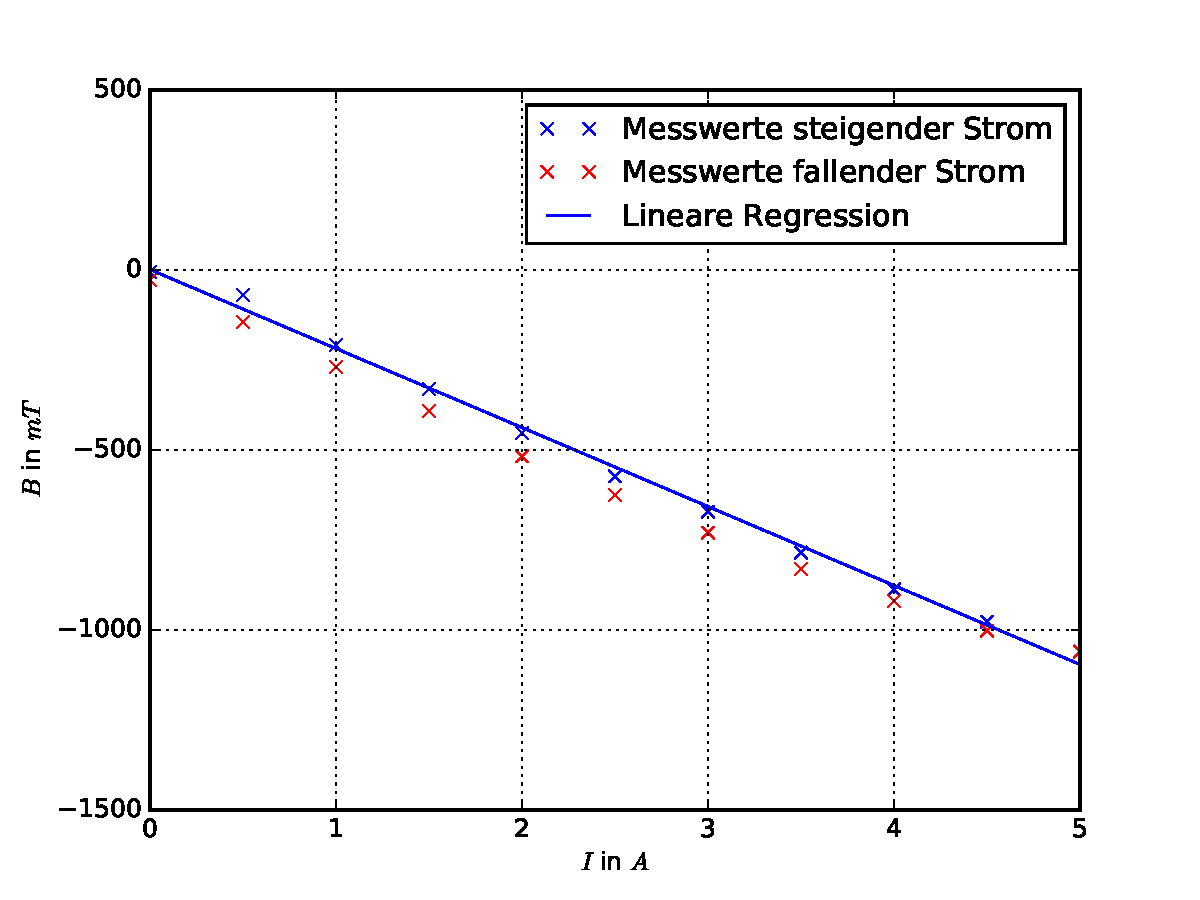
\includegraphics[width=0.7\textwidth]{pics/hysterese.pdf}
  \caption{Verlauf der magnetischen Flussdichte in Abhängigkeit vom Spulenstrom}
  \label{fig: hysterese}
\end{figure}




\subsection{Hallspannung bei konstantem Magnetfeld}
Zur Messung der Hallspannung bei konstantem Magnetfeld wurde für beide Proben der Spulenstrom auf $3\si{\ampere}$ eingestellt. Die
Messwerte für $U_{ges+}$ und $U_{ges-}$ sowie die gemäß \eqref{eq:} berechneten Hallspannungen bei variablem Querstrom sind in den
Tabellen \ref{tab: hall_kupfer_konstB} und \ref{tab: hall_zink_konstB} aufgelistet. Eine weitere Regressionsrechnung ermöglicht mittels Gleichung \eqref{eq: } eine
erste Bestimmung der jeweiligen Teilchenzahl $n$ pro Volumen. Für die Beträge der jeweiligen Steigungen ergeben sich:
\begin{equation}
  m_{Cu} = (1.23 \pm 0.02)\si{\milli \volt \per \ampere}  \quad \quad m_{Zn} = (1.63 \pm 0.24)\si{\milli \volt \per \ampere}%\SI verwenden
\end{equation}
Die Plots befinden sich in den Abbildungen \ref{fig: uh_konstB_kupfer} und \ref{fig: uh_konstB_zink}.
Damit ergeben sich die Werte für die Teilchenzahlen pro Volumen zu:
\begin{equation}
  n_{Cu,1} = (1.85 \pm 0.03)\cdot 10^{26}\,\si{ \meter^{-3}} \quad \quad n_{Zn,1} = (1.68\pm 0.24)\cdot 10^{25}\,\si{ \meter^{-3}}%\SI verwenden
\end{equation}
\begin{table} 
 \centering 
 \begin{tabular}{S S S S } 
 \toprule  
 {$I$ in $\si{\ampere}$} & {$U_{ges-}$ in $\si{\milli \volt}$}  &  {$U_{ges+}$ in $\si{\milli \volt}$} & {$U_{H}$ in $\si{\milli \volt}$} \\ 
\midrule  
 0.0 & -0.336 & -0.338 & -0.001 \\ 
1.0 & -0.338 & -0.337 & 0.001 \\ 
2.0 & -0.340 & -0.336 & 0.002 \\ 
3.0 & -0.341 & -0.335 & 0.003 \\ 
4.0 & -0.343 & -0.335 & 0.004 \\ 
5.0 & -0.345 & -0.334 & 0.005 \\ 
6.0 & -0.346 & -0.333 & 0.006 \\ 
7.0 & -0.348 & -0.332 & 0.008 \\ 
8.0 & -0.350 & -0.331 & 0.009 \\ 
9.0 & -0.351 & -0.331 & 0.010 \\ 
10.0 & -0.353 & -0.330 & 0.011 \\ 
\bottomrule 
 \end{tabular} 
 \caption{Hallspannung Kupfer bei konstantem Magnetfeld} 
 \label{tab: hall_kupfer_konstB} 
  \end{table} %caption bei einer Tabelle drüber setzen und nicht darunter
  \centering
\begin{table} 
 \centering 
 \begin{tabular}{S S S S } 
 \toprule  
 {{$I$ in $\si{\ampere$}} & {{$U_{ges-}$ in $\si{\milli \volt$}}  &  {{$U_{ges+}$ in $\si{\milli \volt$}} & {{$U_{H}$ in $\si{\milli \volt$}} \\ 
\midrule  
 0.0 & -0.339 & -0.339 & 0.000 \\ 
1.0 & -0.426 & -0.429 & -0.002 \\ 
2.0 & -0.517 & -0.520 & -0.002 \\ 
3.0 & -0.603 & -0.610 & -0.004 \\ 
4.0 & -0.692 & -0.699 & -0.004 \\ 
5.0 & -0.777 & -0.795 & -0.009 \\ 
6.0 & -0.870 & -0.885 & -0.008 \\ 
7.0 & -0.959 & -0.975 & -0.008 \\ 
8.0 & -1.045 & -1.064 & -0.010 \\ 
9.0 & -1.128 & -1.151 & -0.012 \\ 
10.0 & -1.220 & -1.261 & -0.020 \\ 
\bottomrule 
 \end{tabular} 
 \caption{Hallspannung Zink bei konstantem Magnetfeld} 
 \label{tab: hall_zink_konstB} 
  \end{table} %caption bei einer Tabelle drüber setzen und nicht darunter
  \centering
\begin{figure}
  \centering
  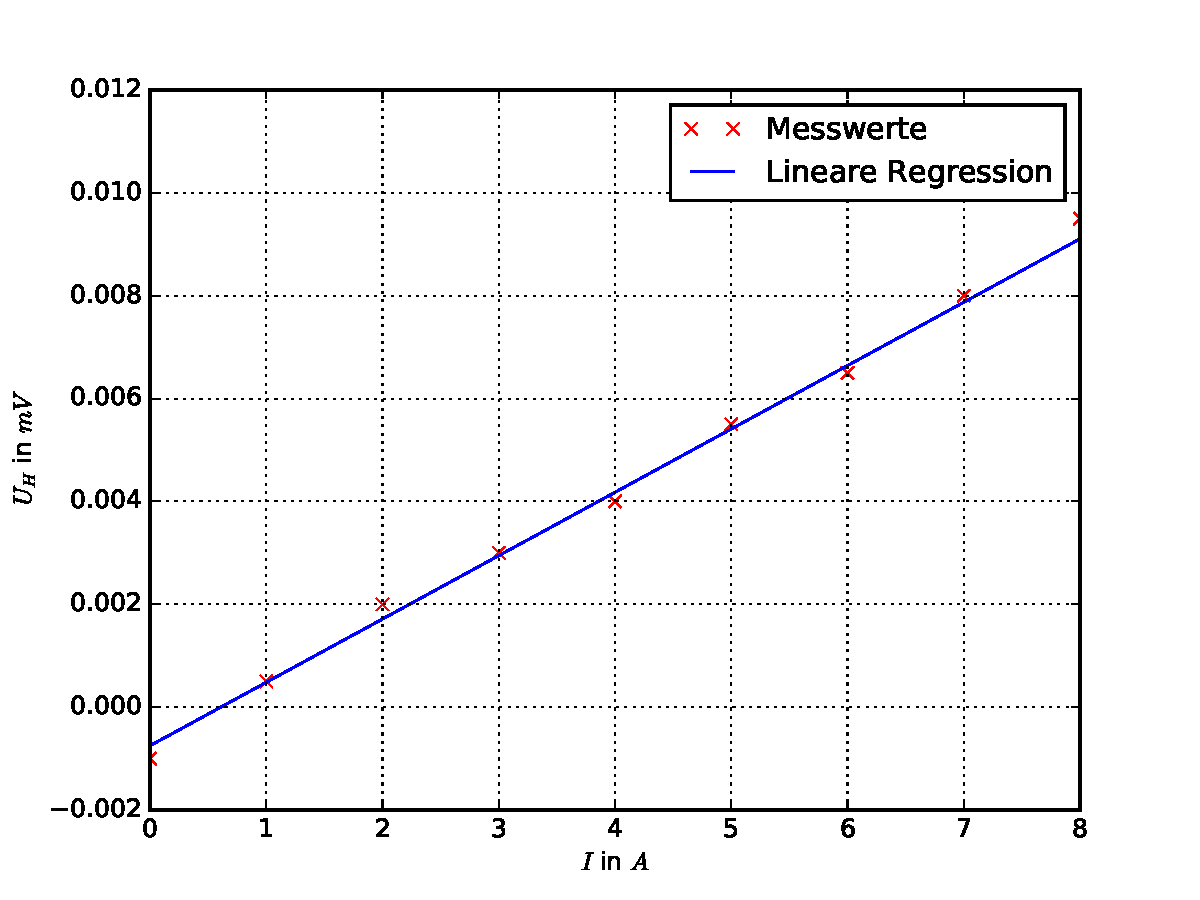
\includegraphics[width=0.7\textwidth]{pics/u_h_kupfer_konstB.pdf}
  \caption{Kupferprobe, Verlauf der Hallspannung in Abhängigkeit vom Querstrom}
  \label{fig: uh_konstB_kupfer}
\end{figure}
\begin{figure}
  \centering
  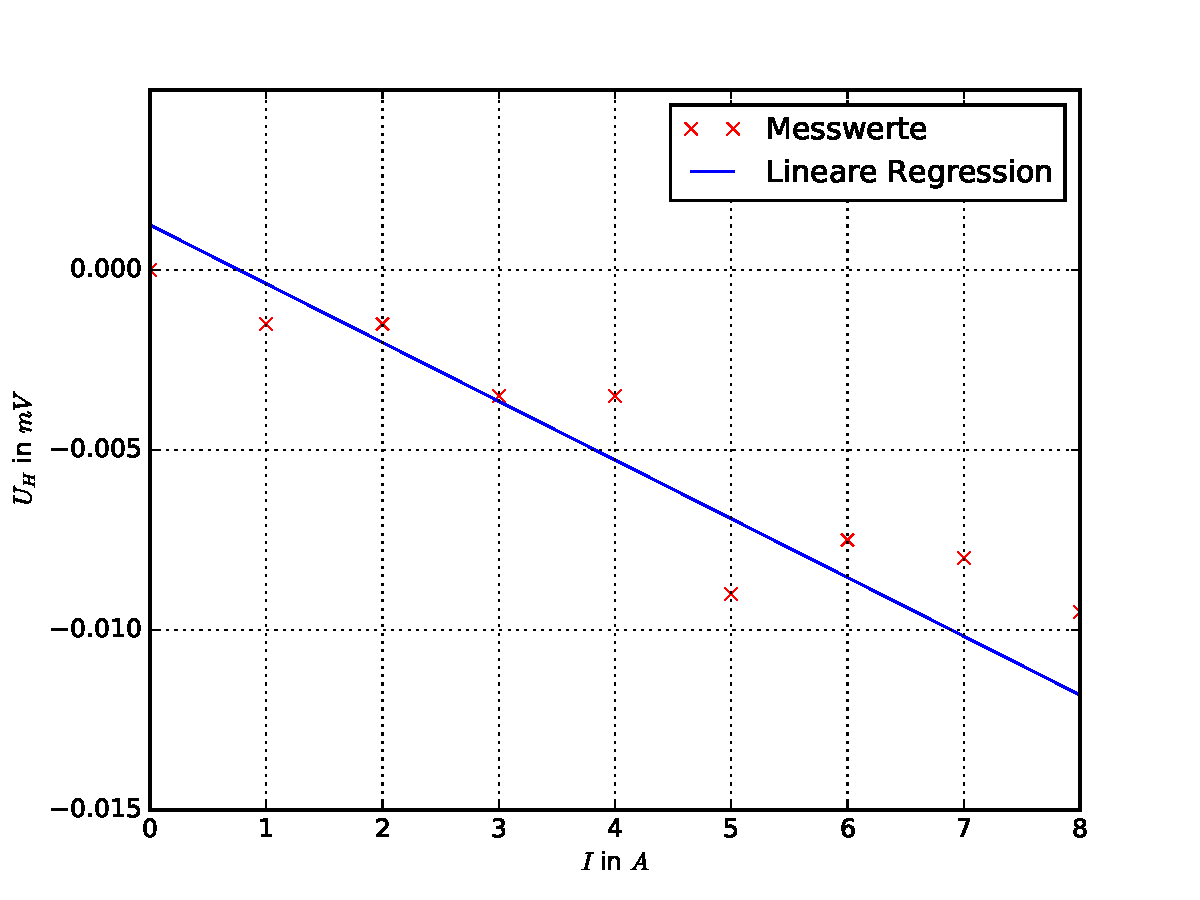
\includegraphics[width=0.7\textwidth]{pics/u_h_zink_konstB.pdf}
  \caption{Zinkprobe, Verlauf der Hallspannung in Abhängigkeit vom Querstrom}
  \label{fig: uh_konstB_zink}
\end{figure}


\subsection{Hallspannung bei konstantem Querstrom}
Zur Messung der Hallspannung bei konstantem Querstrom wurde dieser für beide Proben auf $10\si{\ampere}$ eingestellt. Die%\SI verwenden
Messwerte, sowie die berechneten Hallspannungen sind in den Tabellen \ref{tab: hall_kupfer_konstI} und \ref{tab: hall_zink_konstI} aufgeführt. Dabei wurde
die variable Flussdichte gemäß \eqref{eq: hysterese} berechnet. In den Abbildungen \ref{fig: uh_konstI_kupfer} und \ref{fig: uh_konstI_zink}
wurde der Verlauf der Hallspannung in Abhängigkeit von der Magnetfeldstärke aufgetragen. Für die Beträge der Steigung der Regressionsgeraden
ergeben sich die Werte:
\begin{equation}
  m_{Cu} = (0.018 \pm 0.000)\si{\volt \per \tesla }  \quad \quad m_{Zn} = (0.020 \pm 0.002)\si{\volt \per \tesla}%\SI verwenden
\end{equation}
Der Fehler von $m_{Cu}$ liegt hierbei in der Größenordnung $10^{-17}$. Er wird für folgende Rechnungen jedoch nicht vernachlässigt.
Für die Regression wurde jeweils auf einen Wert verzichtet (Zink $I = 0 \si{\ampere}$, Kupfer $I = 3.5\si{\ampere}$), da diese Werte offenbar%\SI verwenden
durch systematische Fehler beeinträchtigt wurden.\\
Damit ergeben sich die Werte für die Teilchenzahlen pro Volumen zu:
\begin{equation}
  n_{Cu,2} = (1.90 \pm 0.00)\cdot 10^{26}\,\si{ \meter^{-3}} \quad n_{Zn,2} = (2.09\pm 0.16)\cdot 10^{25}\,\si{ \meter^{-3}}%\SI verwenden
\end{equation}
\begin{table} 
 \centering 
 \begin{tabular}{S S S S S } 
 \toprule  
 {$I$ in $\si{\ampere}$} & {$B$ in $\si{\milli\tesla}$} & {$U_{ges-}$ in $\si{\milli \volt}$}  &  {$U_{ges+}$ in $\si{\milli \volt}$} & {$U_{H}$ in $\si{\milli \volt}$} \\ 
\midrule  
 0.0 & 1.1 & -0.340 & -0.324 & 0.008 \\ 
0.5 & -108.6 & -0.341 & -0.340 & 0.001 \\ 
1.0 & -218.2 & -0.343 & -0.338 & 0.003 \\ 
1.5 & -327.9 & -0.345 & -0.336 & 0.004 \\ 
2.0 & -437.6 & -0.347 & -0.334 & 0.006 \\ 
2.5 & -547.3 & -0.349 & -0.332 & 0.008 \\ 
3.0 & -657.0 & -0.351 & -0.330 & 0.010 \\ 
3.5 & -766.7 & -0.353 & -0.328 & 0.012 \\ 
\bottomrule 
 \end{tabular} 
 \caption{Hallspannung Kupfer bei konstantem Querstrom} 
 \label{tab: hall_kupfer_konstI} 
  \end{table} %caption bei einer Tabelle drüber setzen und nicht darunter
  \centering
\begin{table}
 \centering
 \begin{tabular}{S S S S S }
 \toprule
 {$I$ in $\si{\ampere}$} & {$B$ in $\si{\milli\tesla}$} & {$U_{ges-}$ in $\si{\milli \volt}$}  &  {$U_{ges+}$ in $\si{\milli \volt}$} & {$U_{H}$ in $\si{\milli \volt}$} \\
\midrule
 0.0 & 1.1 & -1.195 & -1.264 & -0.034 \\
0.5 & -108.6 & -1.193 & -1.266 & -0.036 \\
1.0 & -218.2 & -1.191 & -1.268 & -0.038 \\
1.5 & -327.9 & -1.189 & -1.272 & -0.041 \\
2.0 & -437.6 & -1.186 & -1.276 & -0.045 \\
2.5 & -547.3 & -1.187 & -1.277 & -0.045 \\
3.0 & -657.0 & -1.185 & -1.279 & -0.047 \\
3.5 & -766.7 & -1.215 & -1.252 & -0.018 \\
\bottomrule
 \end{tabular} 
 \caption{Hallspannung Zink bei konstantem Querstrom}
 \label{tab: hall_zink_konstI}
  \end{table}
 %caption bei einer Tabelle drüber setzen und nicht darunter
  \centering
\begin{figure}
  \centering
  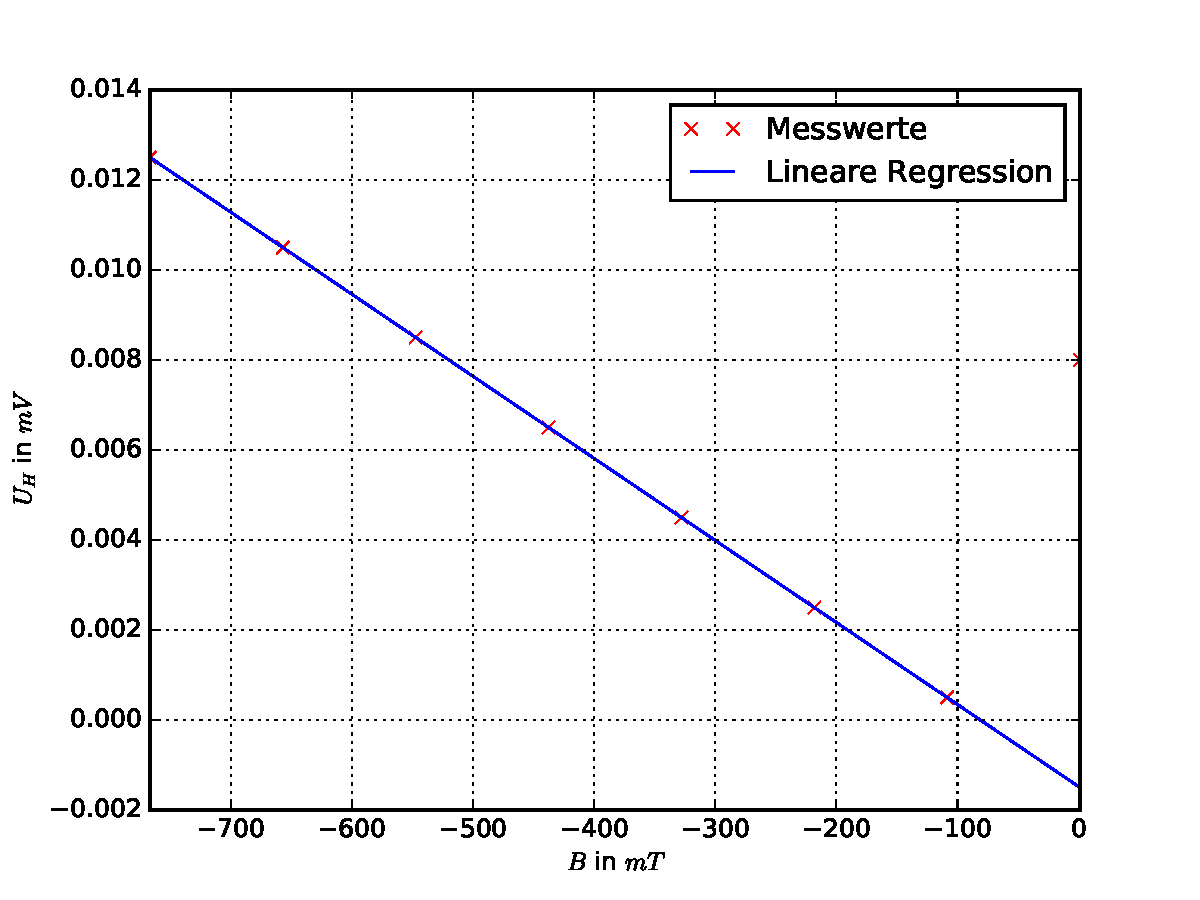
\includegraphics[width=0.7\textwidth]{pics/u_h_kupfer_konstI.pdf}
  \caption{Kupferprobe, Verlauf der Hallspannung in Abhängigkeit von der Magnetfeldstärke}
  \label{fig: uh_konstI_kupfer}
\end{figure}
\begin{figure}
  \centering
  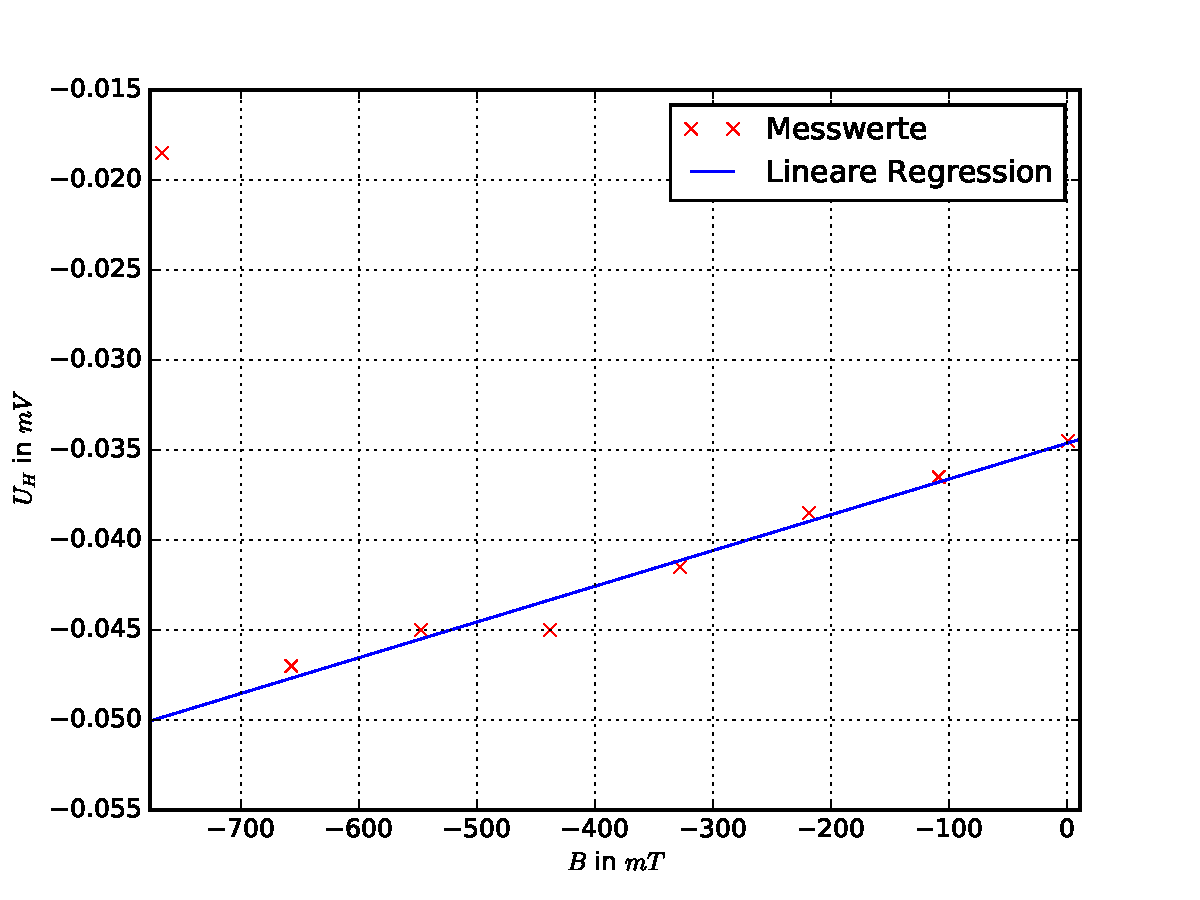
\includegraphics[width=0.7\textwidth]{pics/u_h_zink_konstI.pdf}
  \caption{Zinkprobe, Verlauf der Hallspannung in Abhängigkeit von der Magnetfeldstärke}
  \label{fig: uh_konstI_zink}
\end{figure}


\subsection{Berechnung weiterer Mikroskopischer Größen}
Nun sollen aus den gemessenen makroskopischen Größen auf mikroskopische Zusammenhänge geschlossen werden. Zwischenergebnisse
wurden bei den folgenden Rechnungen nicht gerundet. \\
Mit den molaren Volumina von Kupfer und Zink kann auf die Anzahl der Ladungsträger pro Atom
geschlossen werden. Hierzu wurden die Werte aus V201 \cite{anleitung201} verwendet:
\begin{equation}
  V_{mol, Cu} = 7.09 \cdot 10^{-6} \si{m^3 /mol} \quad   V_{mol, Zn} = 9.16 \cdot 10^{-6} \si{m^3 /mol}%\SI verwenden
\end{equation}
Für Kupfer ergibt sich die Anzahl der Ladungsträger pro Atom zu:
\begin{align}
  \begin{aligned}
    z_{Cu,1} &= n_{Cu,1} \cdot V_{mol, Cu} =  (2.18 \pm 0.04) \cdot 10^{-3}  \\
    z_{Cu,2} &= n_{Cu,2} \cdot V_{mol, Cu} =  (2.24 \pm 0.00) \cdot 10^{-3}
  \end{aligned}
\end{align}
Für Zink berechnen sich die beiden Werte:
\begin{align}
  \begin{aligned}
    z_{Zn,1} &= n_{Zn,1} \cdot V_{mol, Zn} =  (2.5\pm 0.4)\cdot 10^{-4}\\
    z_{Zn,2} &= n_{Zn,2} \cdot V_{mol, Zn} =   (3.2\pm 0.3)\cdot 10^{-4}
  \end{aligned}
\end{align}
Mittels der Abmessungen der verwendeten Leiter kann auf die spezifischen Widerstände der Proben geschlossen werden. Es ergeben sich folgende Werte:
\begin{align}
  \begin{aligned}
    \rho_{Cu} &=  (12.41 \pm 0,03)\cdot 10^{-2} \si{\ohm \milli \meter^2 \per \meter} \\%\SI verwenden
    \rho_{Zn} &=  (69.3 \pm 0,5) \cdot 10^{-2} \si{\ohm \milli \meter^2 \per \meter}
  \end{aligned}
\end{align}
Zusammen mit den gefundenen Werten für die Anzahl der Ladungsträger pro Volumen berechnen sich die mittleren Flugzeiten $\tau_i$ zu:
\begin{align}
  \begin{aligned}
    \tau_{Cu,1} &= (3.09 \pm 0.06) \cdot 10^{-12} \si{\second} \\%\SI verwenden
    \tau_{Cu,1} &= (3.01 \pm 0.00) \cdot 10^{-12} \si{\second} \\
    \tau_{Zn,1} &= (6.1 \pm 0.9) \cdot 10^{-12} \si{\second} \\
    \tau_{Zn,2} &= (4.9 \pm 0.4) \cdot 10^{-12} \si{\second}
  \end{aligned}
\end{align}
Nun soll die Driftgeschwindigkeit $v_d$ für eine Stromdichte von $j = 1 \si{\ampere \per \milli \meter}$ berechnet werden. Mittels Formel
\eqref{eq: } ergeben sich die Werte:
\begin{align}
\begin{aligned}
v_{Cu,1} &= (33.7 \pm 0.6)   \si{\milli\meter\per\second}  \\%\SI verwenden
v_{Cu,2} &= (32.8 \pm 0.00)  \si{\milli\meter\per\second}  \\
v_{Zn,1} &= (3.70 \pm 0.50)\cdot 10^{ 2}   \si{\milli\meter\per\second} \\
v_{Zn,2} &= (1.98 \pm 0.20)\cdot 10^{ 2}   \si{\milli\meter\per\second}
\end{aligned}
\end{align}

Weiter berechnen sich gemäß \eqref{eq:} die Fermi-Energien der Stoffe zu: %soll ich das weglassen?
\begin{align}
\begin{aligned}
E_{Cu,1} &= (11.84 \pm 0.14)\cdot 10^{-3} \, \si{\eV}  \\%\SI verwenden
E_{Cu,2} &= (12.06 \pm 0.00)\cdot 10^{-3} \, \si{\eV}  \\
E_{Zn,1} &= (2.39 \pm 0.23)\cdot 10^{-2}  \,  \si{\eV} \\
E_{Zn,2} &= (2.77 \pm 0.14)\cdot 10^{-2}  \, \si{\eV}
\end{aligned}
\end{align}

Mittels Zusammenhang \eqref{eq: } berechnen sich die Totalgeschwindigkeiten $\left| v \right| $ zu:
\begin{align}
\begin{aligned}
\left|v_{Cu,1}\right| &= (2.04 \pm 0.01)\cdot 10^5 \, \si{\meter \per \second}  \\%\SI verwenden
\left|v_{Cu,2}\right| &= (2.05 \pm 0.00)\cdot 10^5 \, \si{\meter \per \second}  \\
\left|v_{Zn,1}\right| &= (9.20 \pm 0.40)\cdot 10^4 \, \si{\meter \per \second}  \\
\left|v_{Zn,2}\right| &= (9.87 \pm 0.25)\cdot 10^4 \, \si{\meter \per \second}
\end{aligned}
\end{align}

Mit Formel \eqref{eq: } ergeben sich folgende Werte für die mittlere freie Weglänge:
\begin{align}
\begin{aligned}
l_{Cu,1} &= (6.31 \pm 0.08)\cdot 10^{-1} \, \si{\micro\meter}  \\%\SI verwenden
l_{Cu,2} &= (6.19 \pm 0.01)\cdot 10^{-1} \, \si{\micro\meter}  \\
l_{Zn,1} &= (0.56 \pm 0.05) \, \si{\micro\meter}  \\
l_{Zn,2} &= (0.48 \pm 0.03) \, \si{\micro\meter}
\end{aligned}
\end{align}

Die Beweglichkeit $\mu$ ergibt sich schließlich mit \eqref{eq:} zu:
\begin{align}
\begin{aligned}
\mu_{Cu,1} &= (0.27 \pm 0.05) \, \si{\meter^2 \per \volt \second}  \\%\SI verwenden
\mu_{Cu,2} &= (0.26 \pm 0.00) \, \si{\meter^2 \per \volt \second}  \\
\mu_{Zn,1} &= (0.54 \pm 0.08) \, \si{\meter^2 \per \volt \second}  \\
\mu_{Zn,2} &= (0.43 \pm 0.03) \, \si{\meter^2 \per \volt \second}
\end{aligned}
\end{align}
